\vspace{-1cm}
\begin{wrapfigure}[10]{r}{7cm}
  \centering
  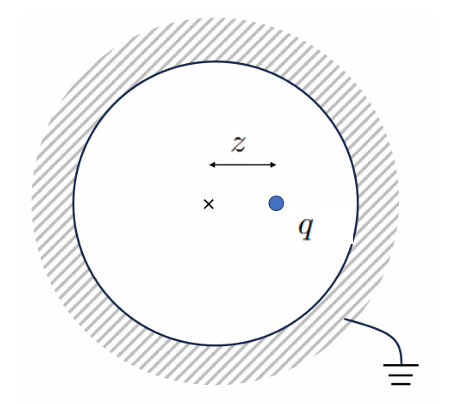
\includegraphics[width=0.4\textwidth]{Figures/Problems/Fig 3.1.png}
  \begin{center}
    \figurename{ 3.1}
  \end{center}
\end{wrapfigure}

\noindent Một quả bóng (có thể xem như điện tích điểm $q>0$) có khối lượng $m$ bị nhốt lại trong một hốc rỗng hình cầu bán kính $R$ được khoét trong một khối điện môi nối đất rất lớn. Điện tích nằm cách tâm hốc cầu một khoảng $z$. Bỏ qua tác dụng của trọng lực.
\begin{enumerate}
  \item Phác hoạ các đường sức điện trường bên trong hốc cầu.
  \item Xác định lực $F(z)$ tác dụng lên quả bóng theo $q, z$ và $R$.
  \item Quả bóng được thả ra tại tâm với vận tốc ban đầu rất nhỏ, tính vận tốc $v$ của quả bóng khi nó cách tâm hốc cầu một khoảng $\dfrac{R}{2}$. Biểu diễn kết quả theo $q, m$ và $R$.
\end{enumerate}